%%%%%%%%%%%%%%%%%%%%%%%%%%%%%%%%%%
% EL/EEE D1 Report Template
% University of Southampton
%
% author : Ben Rowlinson (bdr1g15)
%
% edited : 2017-03-17
%%%%%%%%%%%%%%%%%%%%%%%%%%%%%%%%%%

\documentclass[a4paper,11pt]{article}

%%%%%%%%%%%%%%%%%%%%%%%%%%%%%%%%%%
% PACKAGES
%%%%%%%%%%%%%%%%%%%%%%%%%%%%%%%%%%
\usepackage[margin=1in]{geometry}
\usepackage{amsmath}
\usepackage{graphicx}
\usepackage{wrapfig}
\usepackage[final]{pdfpages}
\renewcommand{\baselinestretch}{1.2} % line spacing
\usepackage{nomencl}
\makenomenclature

%%%%%%%%%%%%%%%%%%%%%%%%%%%%%%%%%%
% DOCUMENT BEGIN
%%%%%%%%%%%%%%%%%%%%%%%%%%%%%%%%%%
\begin{document}
  
\begin{center}
{\Large{\textbf{ELEC2205 D4 -- System Design Exercise}}} \\ [\baselineskip]
Ben Rowlinson\\
bdr1g15\\
MEng Electronic Engineering\\
Dr Yoshishige Tsuchiya\\
17/03/2017\\
\end{center}

\tableofcontents
\newpage
\listoffigures
\newpage
\mbox{}
\nomenclature{IMU}{Inertial Measurement Unit}
\nomenclature{PDB}{Power Distribution Board}
\nomenclature{DMP}{Digital Motion Processing}
\nomenclature{YPR}{Euler Angles: Yaw, Pitch, Roll}
\nomenclature{TYPR}{Throttle, Yaw, Pitch, Roll}
\nomenclature{PID}{Proportional, Integral and Differential control}
\nomenclature{LiPo}{Lithium Polymer}
\nomenclature{UAV}{Unmanned Aerial Vehicle}
\nomenclature{DMM}{Digital Multimeter}
\nomenclature{ESC}{Electronic Speed Controller}
\nomenclature{PSU}{Power Supply Unit}
\printnomenclature
\newpage

\section{Contribution}
As team leader, my contribution to the project was more administrative than hands-on, however did include integrating all the design modules together. I gave myself some smaller auxiliary roles involving tuning the PID controller, interfacing the IR sensor, managing power distribution, and measuring battery voltage. In addition to these roles I was involved to some degree in the development of every design module to ensure tasks were being completed successfully and would integrate smoothly, with minimal fault-finding required.\\ 
For reference, full critical system integration is identified as: The Communications module sending instructions over a radio channel to an on-board receiver, which buffers and forwards the data to the control element, on request. The control element processes these and the IMU data to afford control to the motors.\\
 
\section{Specification}
\subsection{Communications and Control Integration}
The communications and control modules need to fit together seamlessly so that the correct operation of both systems is not affected. The packet transmission time should not exceed 3ms to ensure that neither system is slowed too much by the interface.
\subsection{PID Tuning}
The PID gains of the controller for all three axes of rotation (Yaw, Pitch, Roll) must be tuned such that drone maintains stable flight for and responds accurately to the pilot's input.
\subsection{Power Distribution}
Every component on-board must be correctly powered from a single LiPo battery, via a Power Distribution Board. The controller must be powered by a USB supply from a Laptop.
\subsection{IR Proximity Sensor}
The IR Sensor must accurately measure the current altitude within its operating range (15 to 100cm) to aid the pilot in landing and cargo acquisition manoeuvres.

\section{Design and Simulation}
\subsection{Communications and Control Integration}
The main point of intersection between the communications and control sub-systems, is the UART interface between the on-board Il Matto and Arduino Leonardo boards. This interface is difficult to achieve without causing each of the sub-systems to become too laggy to effectively control the UAV. In this set-up we took the control system to be more critical to the safe operation of the UAV. As such, the Leonardo board was made the 'Master' in this interface so it could request new TYPR (Throttle Yaw Pitch Roll) values when desired.

 The Il Matto would interrupt, set a flag, and send the TYPR packet at the next available opportunity. This has to happen 100 times per second to match the IMU data rate. This process is shown in the control flow diagram.

*** INSERT CONTROL FLOW DIAGRAM ***

Our packet format was dictated by the fact that the serial library chosen could only transmit 8-bit bytes plus 1 start and 1 stop bit. To simplify the receiving procedure we constructed a 17-byte packet format of 'txxxyxxxpxxxrxxx$\backslash$n'

The chars 't', 'y', 'p' and 'r' are identifiers. 'x' is a char 0-9 with the 10-bit ADC value from the X-Y potentiometers being represented by "xxx". The packet is closed by a newline character '$\backslash$n'. The Arduino then leaves the receiving function. As an aside, the ADC values only range from 256 to 768 therefore only "xxx" is needed to represent the full range of ADC values. This is by no means an optimal solution but significantly eases the receiving procedure, as the string can be read in 1 char at time and the values simply assigned to the correct TYPR value. A similar procedure could be used to update PID gain values, but we were unable to implement this feature fully.  

The protocol could not have packets which exceeded 3ms in time. We initially tested with a baud rate of 9600, however we found this to be too slow to transmit the 17 byte packets (One packet took ~17.71ms @ 9600). Switching to a baud rate of 57600 we were able to transmit a packet in 2.95ms. We attempted faster baud rates but the data was more likely to be corrupted so 57600 was settled on.
\subsection{PID Tuning}
In order to gauge how to tune our PID controller, we researched PID gain values for similar Quad-copter configurations, as well as the methods for fine tuning the control. Since the PID gains vary considerably from one drone to the next, these researched values were used as initial 'ballpark' values which we would later refine during the tuning stage. We wanted to implement a feature which would allow us to update PID gains 'on the fly' but we were not able to get this to function correctly.
\subsection{Power Distribution}
For power distribution we wanted to use a single 11.1V 3s LiPo battery to power all on-board components. This required a PDB with could handle the current spikes due to rapid changes in thrust but also supply a smooth 5V to the Arduino and Il Matto. The Il Matto already contains a 3V3 voltage regulator which needs a minimum 4.5V input to operate correctly. The current requirements on the PDB meant I had to supplement the tri-pad board with an additional cable and solder. This ensured we could safely operate the motors at high thrust without damaging the LiPo or the rest of the UAV. Of course this extra cable added weight to the drone. 
\subsection{IR Proximity Sensor}
The IR sensor has proprietary chip which handles the signal processing involved in estimating the distance. This module then outputs an analogue voltage when powered. This means the IR sensor effectively acts like potentiometer. I wrote a test program which performs a 10-bit ADC conversion and outputs the ADC value over a UART interface to the PuTTY terminal. The ADC value is not the actual distance so must be converted to a distance in cm. The approximate relation is ***INSERT IR SENSOR EQN M'HERE WITH REFERENCE TO THE DATASHEET***. This relation can vary from sensor to sensor so a calibration routine must be implemented to be able to collect reasonable data.
\subsection{Schematic}
As part of the design process I compiled our design plan into a high-level block diagram and later an EAGLE schematic of the complete electronic design. This EAGLE schematic allowed us to accurately plan out our on-board layout and ensure that we had enough power connections for every component. This schematic was also used as a reference by the team to ensure consistent assembly of the circuitry. (Appendix C of Team Report)



\section{Testing and Results}
\subsection{Communications and Control Integration}
By consulting the communications and control sub-system teams, to see what they wanted from the interface, I wrote a test program investigating each side of the interface to verify the operation and speed of this protocol. These results show that the used Baud Rate of 9600 is too slow to ***SOMEWHERE-INSERT SCOPE CAPTURE"***. This meant that, when we were able to do the critical path test, I could simply add my interfacing program to the existing communications and control sub-systems, knowing that it already worked correctly.
\subsection{PID Tuning}
Initially, our approach to testing our fully integrated UAV was to tether it down and throttle it to see if it could enter a stable flight. This testing method proved fruitless as the UAV was never under its own control, but instead was influenced by the tethering set-up.
***INSERT TETHERED SETUP PICTURE M'HERE***
 We concluded that we ought to let the drone fly free of tethers in a wide open space. Unfortunately, this led to the back legs and feet snapping off a number of times due to a consistent pitch backwards on take-off. We re-evaluated our approach to tuning the PID controller. Instead of trying to tune all the axes of rotation concurrently, we decided to suspend the drone such that only one axis was rotated around (Dubbed Balance testing).
***INSERT INITIAL BALANCE TESTING PIC***
  The centre of mass was initially placed (wrongly) below the axis of rotation leading to incorrect PID values. We realised this error and continued testing with the centre of mass now above the axis of rotation. This gave us an inherently more unstable initial condition, which offered a better test of the control.
***INSERT FINAL BALANCE TESTING PIC***
   Again, we saw the consistent pitch backward being exhibited by the drone. After an exhaustive debugging procedure we concluded that the problem lay in one of the ESCs being un-calibrated with respect to the other three and as such never provided the balanced thrust required to maintain stable flight. After this was rectified we contained with the balance testing, to great effect.
***INSERT PICTURE SHOWING SUCCESSFUL BALANCE TEST***
    We were able to perform tuning of the Pitch and Roll PID values but were unable to tune the Yaw control, or indeed do a full flight test, before the final hand-in.
\subsection{Power Distribution}
 Initially to verify the correct operation of the PDB I used a bench DMM to check for continuity errors, then powered the ESCs without motors connected. The 5V regulator was then added and again tested using the above procedure, with the Arduino and Il Matto boards instead of the ESCs. Next, I performed a full power distribution test with all components connected, using a current limited (500mA) PSU to protect from unexpected current surges, but without driving the motors. Following these successful tests I powered all the components including the motors simultaneously, again with a current limit (5A). Finally a full PDB test with the LiPo battery was performed which was successful on the first test, as expected.
\subsection{IR Proximity Sensor}
To calibrate the IR sensor very roughly I placed a planar surface at 75cm from the sensor, measured the ADC value at that distance, then scaled the conversion to the desired value (75cm). This gave us a reasonably good approximation of the current altitude, if the drone was below 1m in altitude. To improve our altitude measuring capabilities we could have included an ultra-sound module but our research showed that the very noisy environment created by the motors severely affects the the accuracy of the ultrasound modules. Another option could be using a barometric sensor to detect altitude change due to changing air pressure. 


\section{Management and Team Working}
\subsection{Approach to Management}
As team leader, my approach to managing the team was to designate specific roles to the team as early on as possible, whilst ensuring everyone was content with their role and place in the team. Built into this strategy was a sense of redundancy, in that no one was solely responsible for a particular sub-system. This meant that if a team member was away from meetings or working sessions, we would still be able to discuss problems reasonably well. Fortunately the entire team was very responsive to this and were consistent in attending meetings and lab time. We worked cohesively as a single unit throughout the duration of the project with no personal conflicts or arguing. The only disagreements were due to different approaches to the same engineering problem, which lent itself to a very healthy working environment. I felt it was important that the team met and worked together face-to-face at every opportunity, but also allowed for a period of time away from the project. 
\subsection{Designating Technical Roles}
After a couple of days of initial research into the project, it became clear who was suitable for certain roles within the team. I partitioned the team such that one pair was responsible for communications (J Trickey and M Ibrahim) and another pair (L Gray and J Hindmarsh) were responsible for control. I worked closely with both pairs throughout the project, with them consulting me to ensure consistency in the design and keeping me up to date with their progress. This included resolving any issues quickly and efficiently. This meant when we came to integrate modules together I already had a firm grasp of the entire system functionality, easing the integration process.
\subsection{Management Roles}
I designated the team to complete various administrative roles within the team which would continue throughout the project. These included Treasurer(L Gray), Minutes(J Trickey), Documentation/Photography(M Ibrahim) and external communications(J Hindmarsh). Each of the team members had these auxiliary roles to fulfil.
\subsection{Project Planning}
With regard to the planning process we identified this as the critical path for the construction of the drone electronics, that would enable basic functionality. Up until the point we could perform a full critical system integration, we worked on some of the extra functions if and only if the critical task had already been performed. We planned for full critical system integration to be finalised on Thursday 9th March and from that point onwards we would concentrate on tuning our PID controller and adding extra functionality if possible.
\subsection{Risk Management}
We drew up a fairly broad risk assessment, based on our intensive research early on in the project. Fortunately, very little went wrong in our approach, that we didn't expect to go wrong. The chassis did shatter a number of times during flight and tethered tests, but we always ensured we were able to bring the drone back to flying condition or left enough time to manufacture a new frame. Any expected long term absences (more than 24hrs) were declared to me by the team in the first few days of the project so we could work around the team members' schedule without compromising the progress of the project.


\section{Critical Evaluation and Reflection}
\subsection{On My Contribution}
 As team leader I felt it was important for me to take a step back and consider the project as a whole rather than focusing too much on performing a particular task but on reflection, I feel that I could have contributed more of my technical skills to the project. What I did contribute technically did however affect the success and functionality of our system.  
\subsection{On the Team's Progress}
The team did good
\subsection{On Management}
In conclusion, with regard to my managerial approach, I would say that it was a true pleasure to manage such a dedicated, motivated, and intelligent team. We always worked together as a unit. They made my experience on the project very enjoyable.
\subsection{Overall Reflections}
Overall, I am pleased with how we developed the project. Although we were not able to sustain a stable flight in the testing phase, the process we went through to get to that stage was challenging and fulfilling. 
Retrospectively, we should have re-evaluated our approach to flight testing procedure, and approached it in a more structured and thoughtful way.




\appendix
\newpage
\section{References}
Hello

\section{Figures}
Here are some figures
\setboolean{@twoside}{false}
\begin{figure}[!h]
    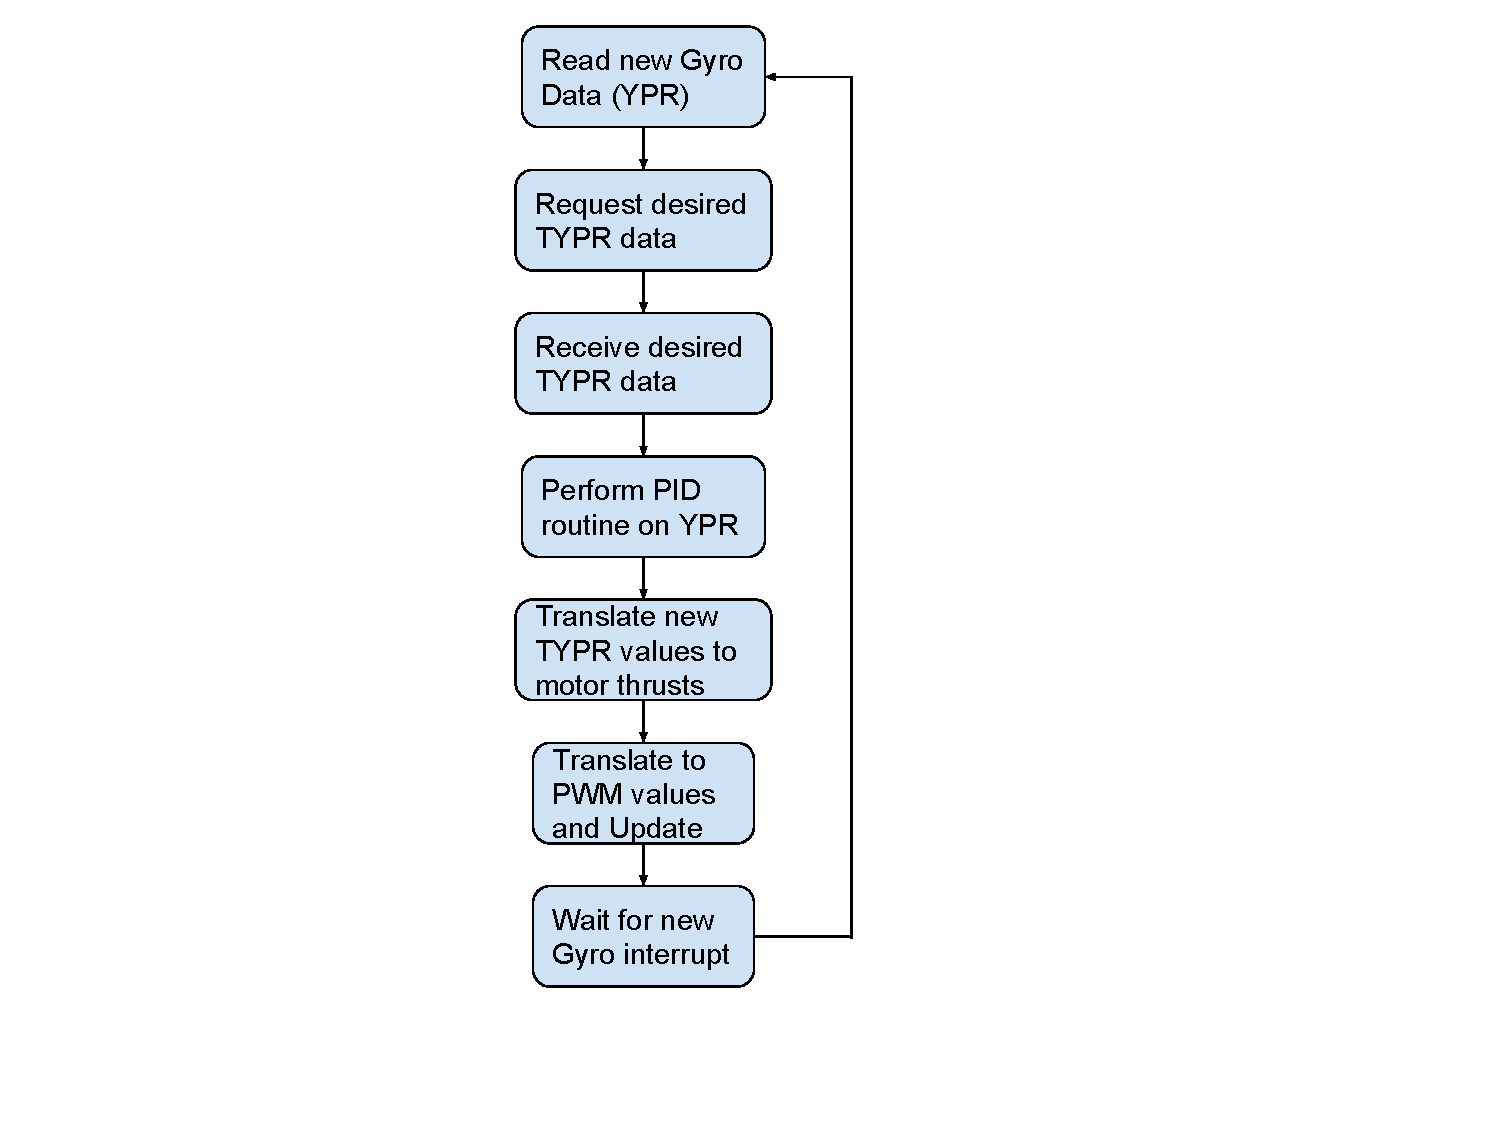
\includepdf[pages=-,pagecommand={},width=\textwidth]{D4-Ganges_Control_flow_diagram.pdf}
    \caption{Diagram showing the flow of control in the Control Micro-controller}
    \label{fig:Control Flow}
\end{figure}
\newpage
\begin{figure}[!h]
    \includepdf[pages=-,pagecommand={},width=\textwidth]{onboard_v1_1.pdf}
    \caption{Full Schematic REMOVE LATER}
\end{figure}

  
\end{document}